\chapter{Obiecte de Tip Dimensiune}
\label{sec:obiecte_dimensiune}

\section{Dimensiunea temporală: dim\_time\_dim}

Obiectul \texttt{dim\_time\_dim} se bazează pe tabelul \texttt{DIM\_TIME} și definește:

\begin{itemize}
    \item \textbf{Nivele:} \texttt{zi\_lvl} (date\_key), \texttt{saptamana\_lvl} (an, saptamana\_an), \texttt{luna\_lvl} (an, luna), \texttt{trimestru\_lvl} (an, trimestru), \texttt{an\_lvl} (an).
    \item \textbf{Ierarhia comercială} (\texttt{commercial\_hier}): zi $\rightarrow$ săptămână $\rightarrow$ an (pentru analize pe săptămâni din an).
    \item \textbf{Ierarhia calendar} (\texttt{calendar\_hier}): zi $\rightarrow$ lună $\rightarrow$ trimestru $\rightarrow$ an (pentru drill-down lunar/trimestrial).
    \item \textbf{Atribute:} \texttt{zi\_lvl} determină \texttt{data\_completa}, \texttt{zi\_saptamana\_nume}, \texttt{este\_weekend}; \texttt{luna\_lvl} determină \texttt{luna\_nume}, \texttt{luna\_abrev}.
\end{itemize}

\section{Dimensiunea topic: dim\_topic\_dim}

Obiectul \texttt{dim\_topic\_dim} se bazează pe tabelul \texttt{DIM\_TOPIC} și definește:

\begin{itemize}
    \item \textbf{Nivele:} \texttt{topic\_lvl} (topic\_key), \texttt{type\_lvl} (topic\_type).
    \item \textbf{Ierarhia} (\texttt{topic\_hier}): topic $\rightarrow$ tip (serviciu/produs).
    \item \textbf{Atribute:} \texttt{topic\_lvl} determină \texttt{nume}, \texttt{descriere}, \texttt{tip\_serviciu}, \texttt{versiune}.
\end{itemize}

\section{Validarea dimensiunilor}

În imaginile urmatoare se poate observa verificarea dimensiunilor si validarea lor.

\begin{figure}[H]
    \centering
    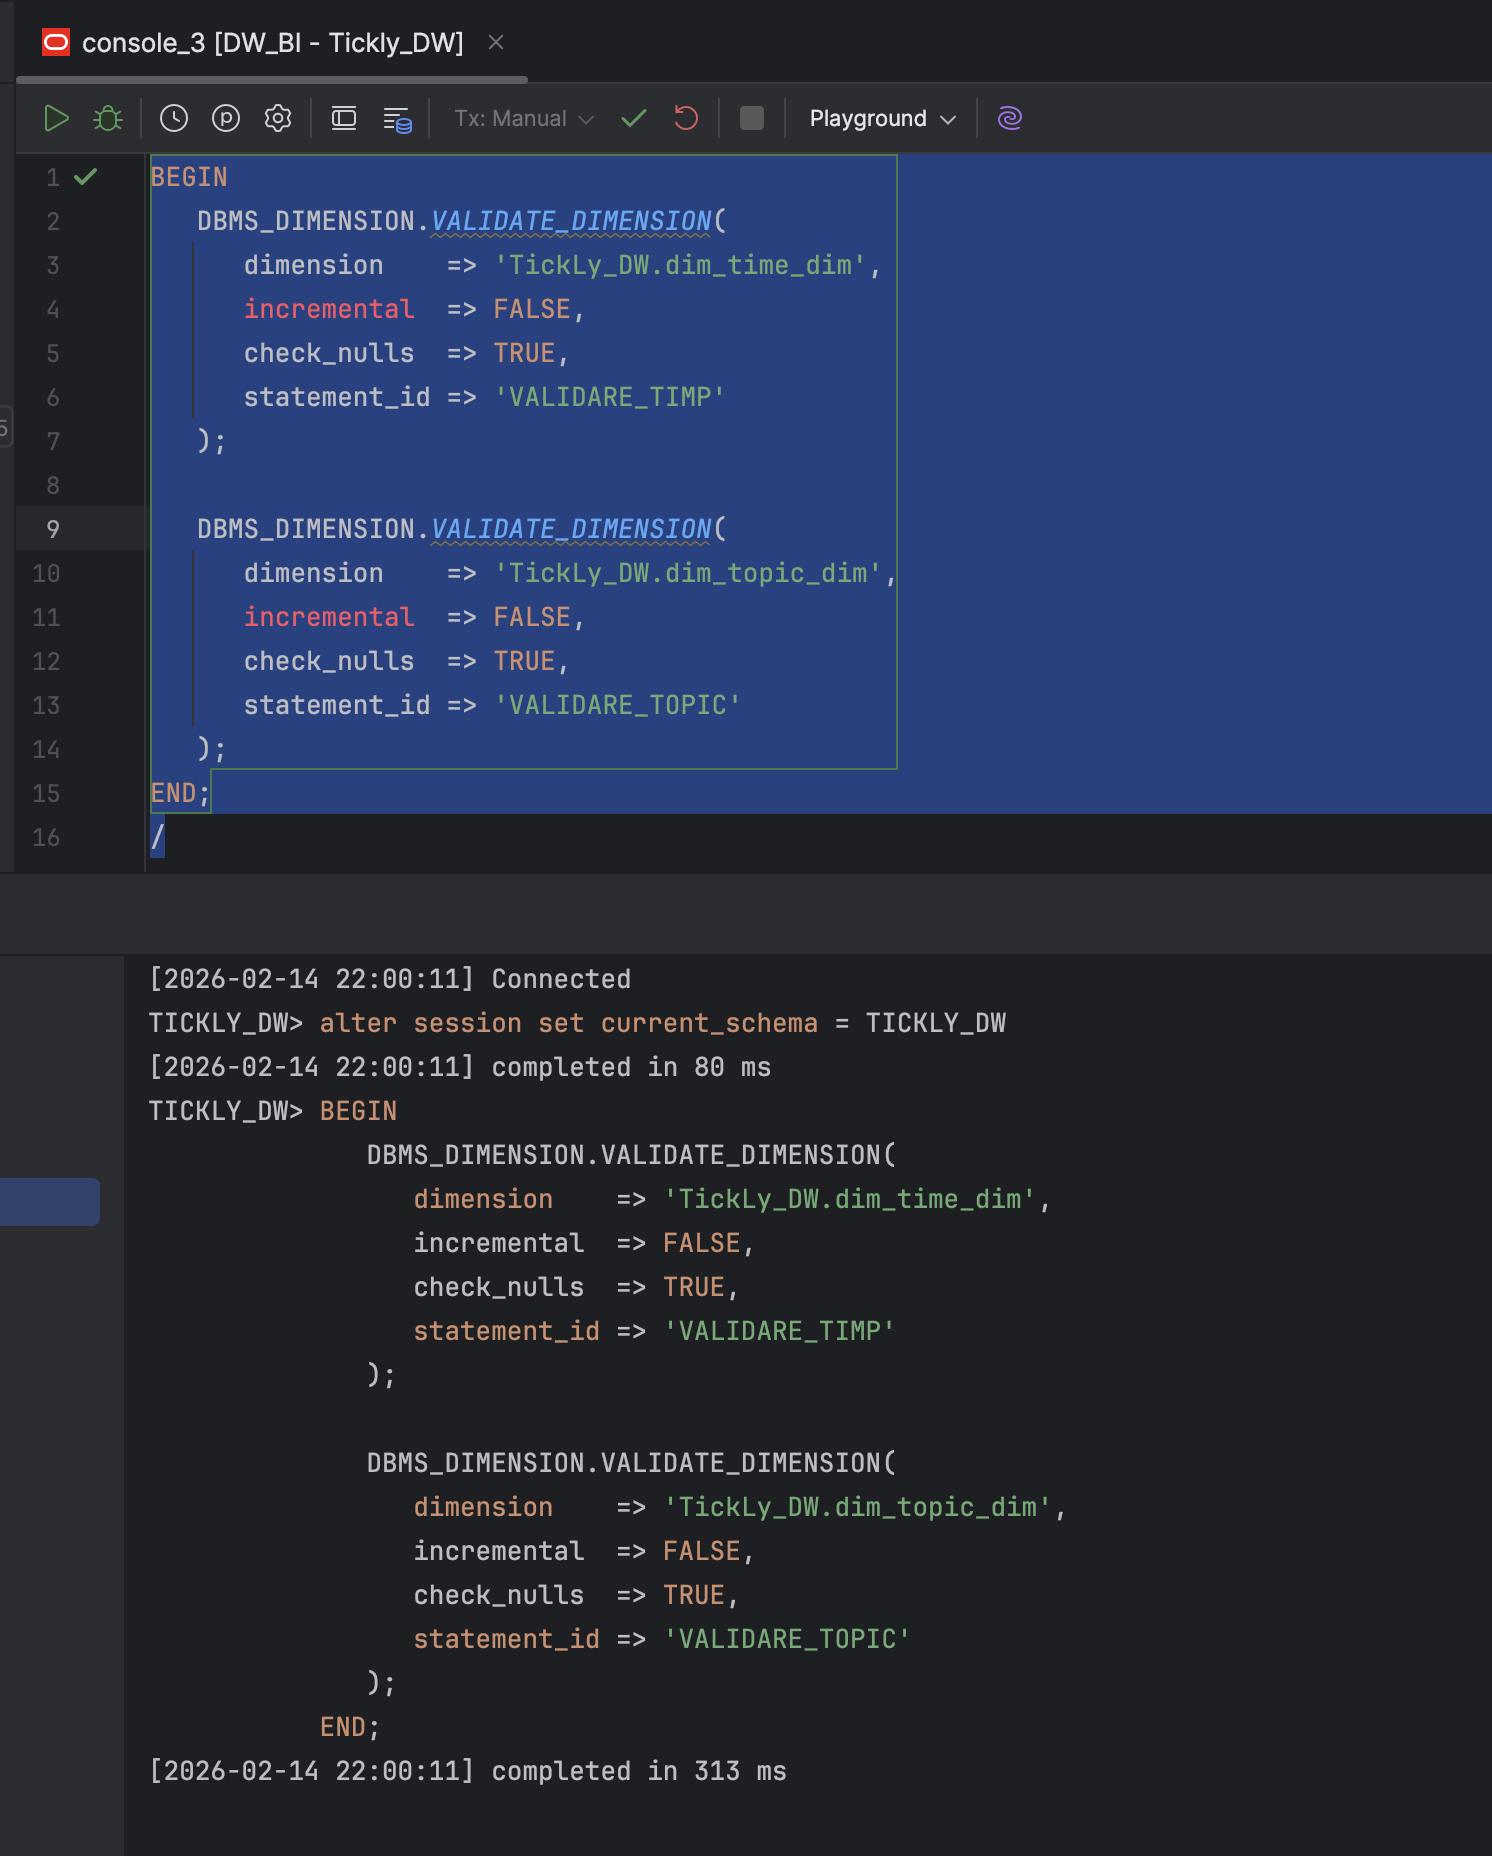
\includegraphics[width=0.6\textwidth]{../../scripts/tests/assets/validare_dimensiune.png}
    \caption{Validarea dimensiunilor}
    \label{fig:validate_dimensions}
\end{figure}

\begin{figure}[H]
    \centering
    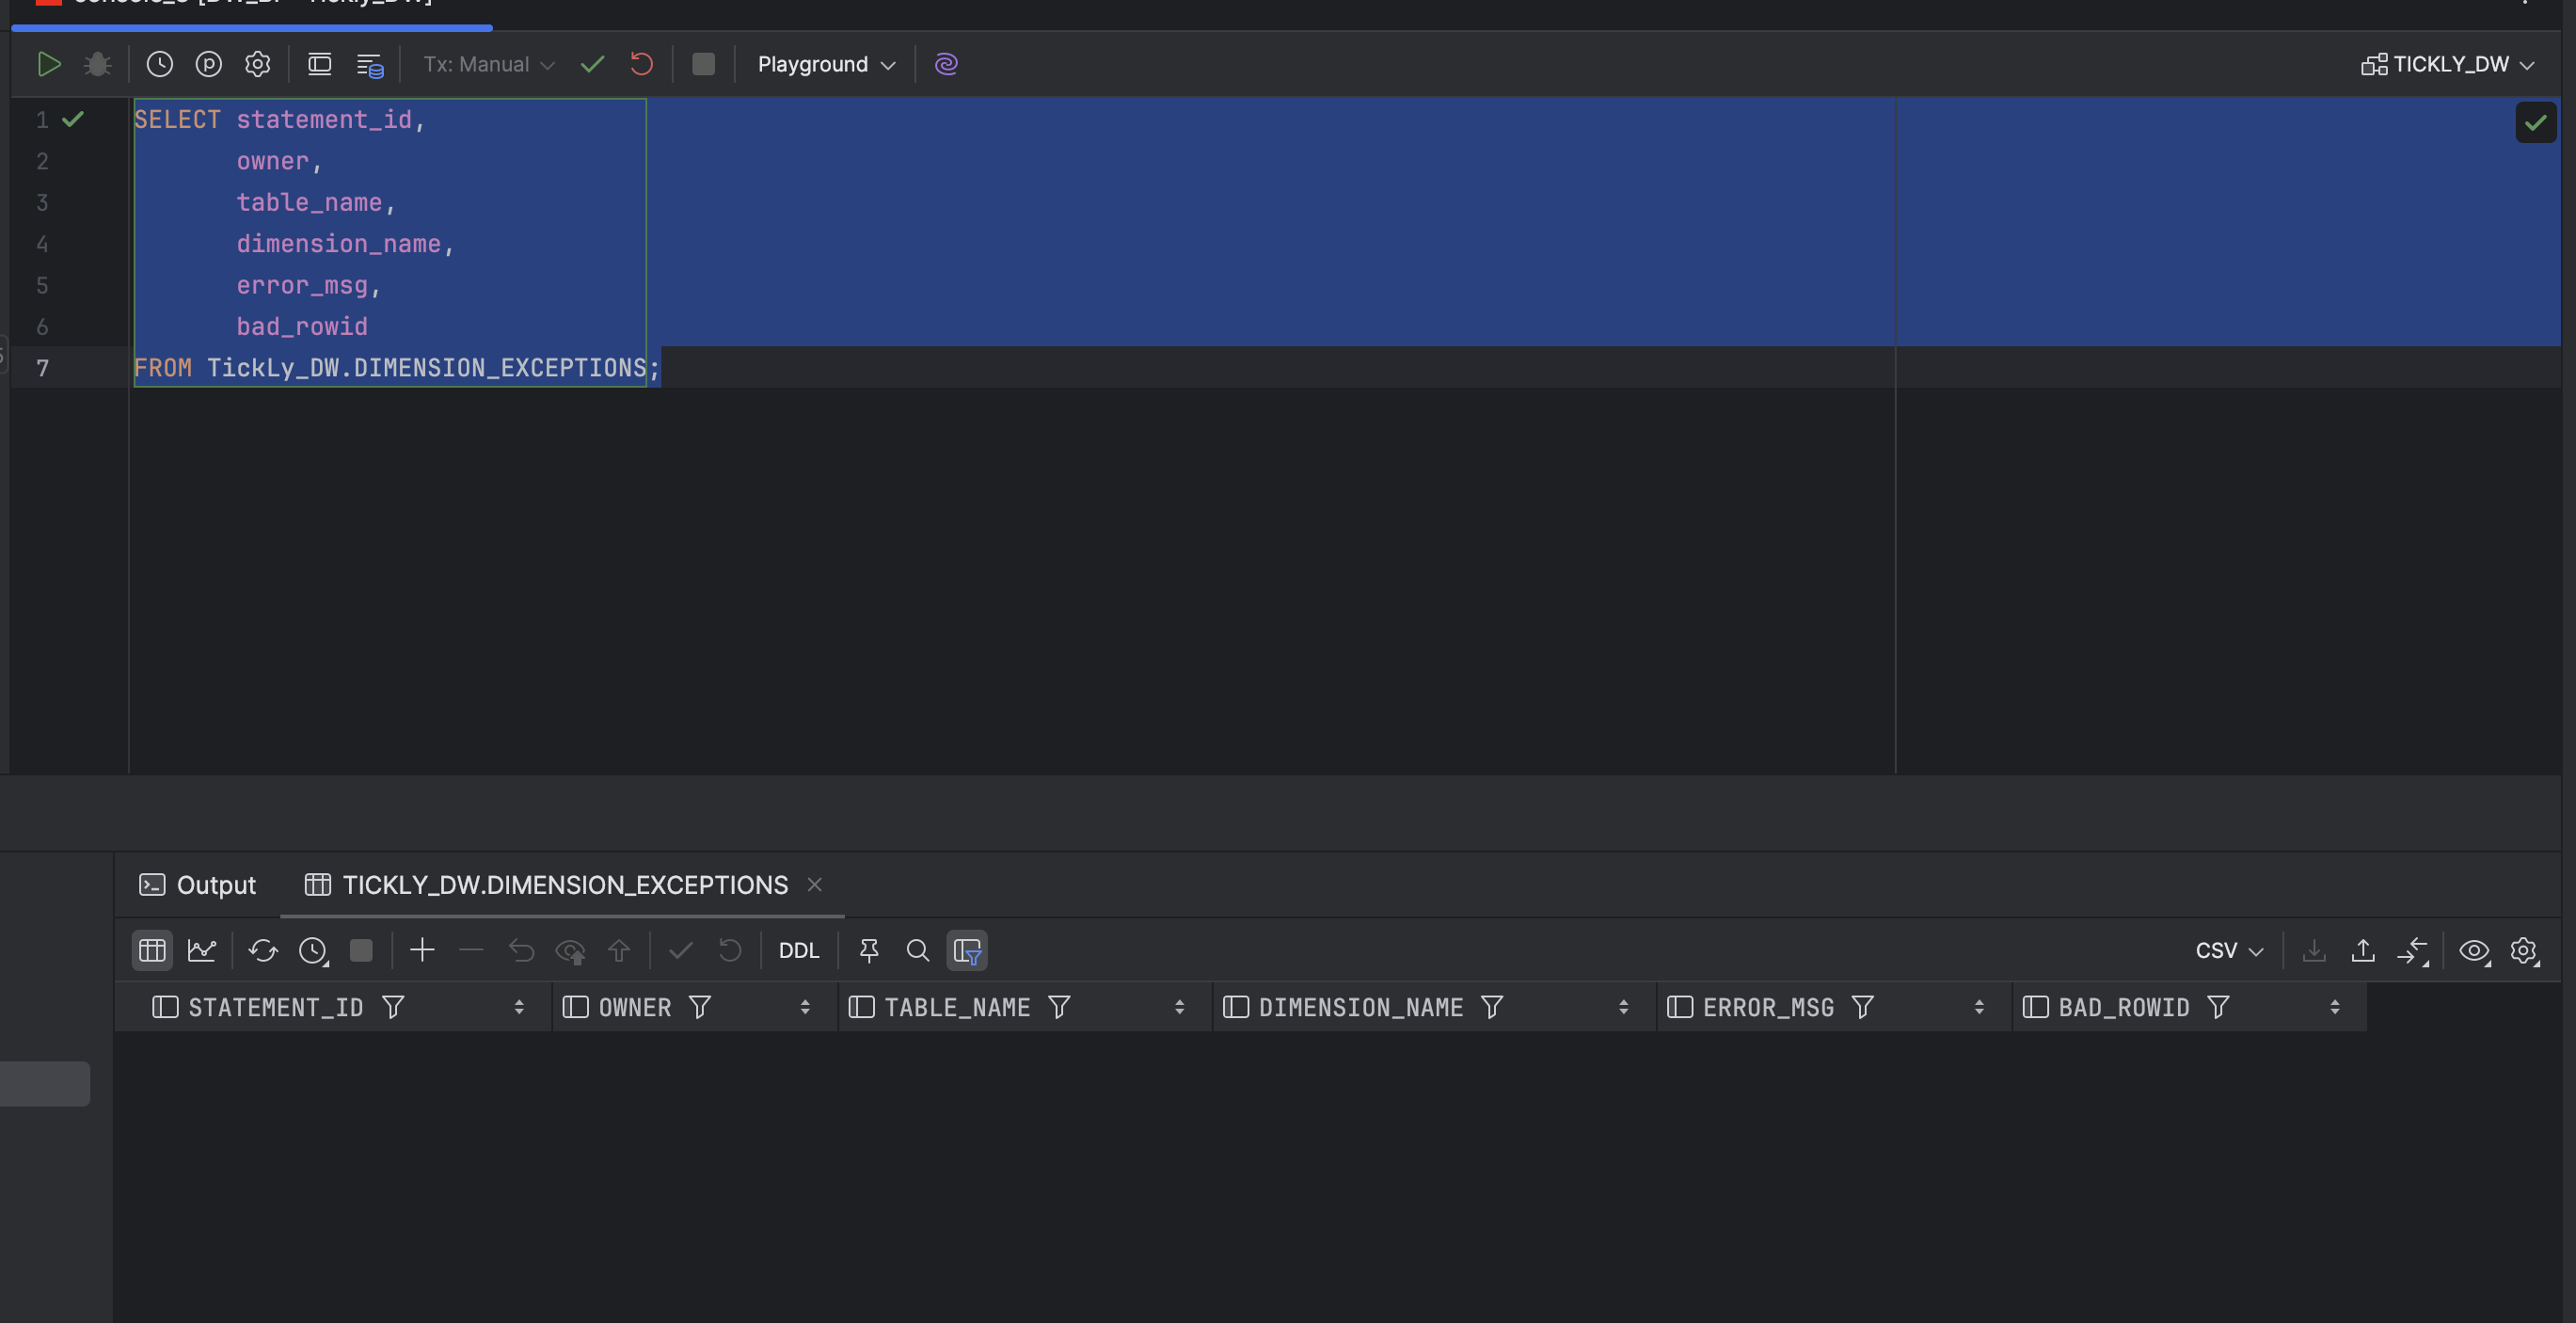
\includegraphics[width=0.6\textwidth]{../../scripts/tests/assets/verificare_validare_dimensiune.png}
    \caption{Verificarea validării dimensiunilor}
    \label{fig:verificare_validare_dimensiune}
\end{figure}
